\documentclass{standalone}
\usepackage{tikz}
\usepackage{ctex,siunitx}
\usepackage{tkz-euclide}
\usepackage{amsmath}
\usetikzlibrary{patterns, calc}
\usetikzlibrary {decorations.pathmorphing, decorations.pathreplacing, decorations.shapes,}
\begin{document}
\small
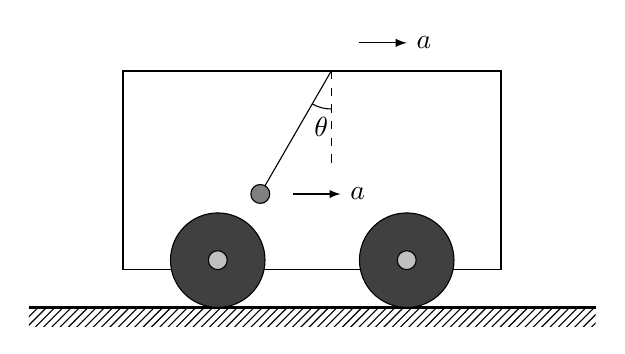
\begin{tikzpicture}[>=latex,scale=1.2]
  \draw[semithick](-1,0.4) rectangle (3,2.5);
  \fill [pattern = north east lines] (-2,-.2) rectangle (4, 0);
  \draw[thick](-2,0)--(4,0);
  \draw[dashed](1.2,2.5)--(1.2,1.5) ;
  \draw (1.2,2.5)--++(240:1.5);
  \draw [fill=darkgray] (0,.5)  circle (0.5);
  \draw [fill=darkgray] (2,.5)  circle (0.5);
  \draw [fill=gray] ([shift=(240:1.5)]1.2,2.5)  circle [radius=.1];
  \draw [->] (0.8,1.2)--++(0.5,0) node [right]{$a$};
  \draw [->] (1.5,2.8)--(2,2.8) node [right]{$a$};
  \draw (1.2,2.1) arc(-90:-120:.4) node [midway,below]{$\theta$};
  \draw [fill=lightgray] (0,.5)  circle [radius=.1];
  \draw [fill=lightgray] (2,.5)  circle [radius=.1];
\end{tikzpicture}
\end{document}